\PassOptionsToPackage{dvipsnames}{xcolor} % https://tex.stackexchange.com/a/653721/258644
\documentclass[25pt, a0paper, portrait]{tikzposter}

% original template: https://rig.cs.luc.edu/~rig/home/tex/tikz/tikzposter-example.tex
%\usepackage{hyperref} % buggy: https://tex.stackexchange.com/questions/165846/incompatibility-between-tikzposter-class-and-microtype-package and https://bitbucket.org/surmann/tikzposter/issues/42/ctan-does-not-have-a-recent-version
\usepackage{url}
\usepackage{amsmath}
\usepackage{amssymb}
\usepackage{graphicx}
\usepackage{svg}
\usepackage{adjustbox}
\usepackage{mathrsfs} % \mathscr
\usepackage{setspace} % \setstretch etc.
\usepackage{csquotes}
\usepackage{fontawesome} % for Github icon
\usepackage{academicons} % for arXiv icon
\usepackage{qrcode}

\usepackage{fontspec}
\setmonofont[Scale=MatchLowercase]{JuliaMono}
\newfontfamily{\emojifont}{Twemoji.Mozilla}[
    Path = ./fonts/,
    Extension = .ttf,
    Renderer = HarfBuzz,
]
\newcommand{\emoji}[1]{{\emojifont #1}}

% itemize bullet styles
%\renewcommand{\labelitemi}{\tiny\blacksquare}
%\renewcommand{\labelitemii}{\color{blue}$\circ$}
\usepackage{enumitem}
\setlist[itemize, 1]{label=\raisebox{0.3ex}[0pt][0pt]{\small$\blacktriangleright$}}

\usepackage{tikz}
\usetikzlibrary{positioning}
\usetikzlibrary{arrows}
\usetikzlibrary{arrows.meta}
\usetikzlibrary{trees}

\usepackage{tcolorbox}
\definecolor{codebg}{HTML}{F8F8F8}
\definecolor{codeframe}{HTML}{D8D8D8}
\newtcolorbox{codeinbox}[1][]{
boxrule = 2pt,
boxsep = 6pt,
colback = codebg,
colframe = codeframe,
fontupper=\normalsize,
#1
}
\newtcolorbox{codeoutbox}{
boxrule = 3pt,
boxsep = 8pt,
colback = white,
colframe = codeframe,
fontupper=\normalsize,
}

% https://tex.stackexchange.com/a/476488
% http://www.numdam.org/item/CG_1998___28-29_158_0.pdf
\usepackage{fancyvrb}
\fvset{formatcom=\setlength{\lineskip}{0pt}}
\begin{SaveVerbatim}{code1}
using SymBoltz
M = ΛCDM()
\end{SaveVerbatim}
\begin{SaveVerbatim}{code2}
equations(M.G)
\end{SaveVerbatim}
\begin{SaveVerbatim}{code3}
p = Dict(
  M.g.h => 0.70, M.γ.T₀ => 2.7, M.c.Ω₀ => 0.27, M.b.Ω₀ => 0.05, M.ν.Neff => 3.0,
  M.b.YHe => 0.25, M.h.m_eV => 0.06, M.I.ns => 0.95, M.I.ln_As1e10 => 3.04
)
prob = CosmologyProblem(M, p)
\end{SaveVerbatim}
\begin{SaveVerbatim}{code4}
ks = range(1.0, 1000.0, length=500) # k / (H₀/c)
sol = solve(prob, ks)
\end{SaveVerbatim}
\begin{SaveVerbatim}{code5}
using Plots
ks_plot = [1.0, 10.0, 100.0, 1000.0]
plot(sol, log10(M.g.a), [M.b.Xe, M.b.rec.XH⁺, M.b.rec.XHe⁺, M.b.rec.XHe⁺⁺])
plot(sol, log10(M.g.a), [M.g.Φ, M.g.Ψ], ks_plot)
plot(sol, log10(M.g.a), [M.ST, 100*M.SE_kχ²], [1.0, 10.0, 100.0, 1000.0])
\end{SaveVerbatim}
\begin{SaveVerbatim}{code6}
ks = 10 .^ range(0, 3, length=100)
Ps = spectrum_matter([:m, :cb, :h], prob, ks)

jl = SphericalBesselCache(25:25:2500)
Cls = spectrum_cmb([:TT, :EE, :ψψ], prob, jl)
\end{SaveVerbatim}
\begin{SaveVerbatim}{code7}
@parameters w₀ wₐ cₛ² Ω₀ ρ₀=3Ω₀/8π
@variables ρ(τ) P(τ) w(τ) cₐ²(τ) δ(τ,k) θ(τ,k) σ(τ,k)
eqs = [
  w ~ w₀ + wₐ*(1-a)
  ρ ~ ρ₀ * a^(-3(1+w₀+wₐ)) * exp(-3wₐ*(1-a))
  P ~ w * ρ
  cₐ² ~ w - 1/(3ℋ) * D(w)/(1+w)
  D(δ) ~ 3ℋ*(w-cₛ²)*δ - (1+w) * ((1+9(ℋ/k)^2*(cₛ²-cₐ²))*θ - 3*D(Φ))
  D(θ) ~ (3cₛ²-1)*ℋ*θ + k^2*cₛ²*δ/(1+w) + k^2*Ψ
  σ ~ 0
]
initialization_eqs = [
  δ ~ -3//2 * (1+w) * Ψ
  θ ~ 1//2 * (k^2*τ) * Ψ
]
X = System(eqs, τ; initialization_eqs, name = :X)
M = ΛCDM(Λ = X, name = :w₀wₐCDM)
\end{SaveVerbatim}
\begin{SaveVerbatim}{eqs_symboltz}
D(Fν0) ~ -k*Fν[1] + 4*D(Φ)
D(Fν[1]) ~ k/3*(Fν0-2Fν[2]+4Ψ)
[D(Fν[l]) ~ k/(2l+1) * (l*Fν[l-1] - (l+1)*Fν[l+1]) for l in 2:lνmax-1]...
D(Fν[lνmax]) ~ k*Fν[lνmax-1] - (lνmax+1) / τ * Fν[lνmax]
δν ~ Fν0
θν ~ 3k*Fν[1]/4
σν ~ Fν[2]/2    
\end{SaveVerbatim}
\begin{SaveVerbatim}{eqs_class}
/** - ---> ultra-relativistic neutrino/relics (ur) */
if (pba->has_ur == _TRUE_) {
    /** - ----> if radiation streaming approximation is off */
    if (ppw->approx[ppw->index_ap_rsa] == (int)rsa_off) {
    /** - -----> ur density */
    dy[pv->index_pt_delta_ur] =
        // standard term
        -4./3.*(y[pv->index_pt_theta_ur] + metric_continuity)
        // non-standard term, non-zero if if ceff2_ur not 1/3
        +(1.-ppt->three_ceff2_ur)*a_prime_over_a*(y[pv->index_pt_delta_ur] + 4.*a_prime_over_a*y[pv->index_pt_theta_ur]/k/k);
    /** - -----> ur velocity */
    dy[pv->index_pt_theta_ur] =
        // standard term with extra coefficient (3 ceff2_ur), normally equal to one
        k2*(ppt->three_ceff2_ur*y[pv->index_pt_delta_ur]/4.-s2_squared*y[pv->index_pt_shear_ur]) + metric_euler
        // non-standard term, non-zero if ceff2_ur not 1/3
        -(1.-ppt->three_ceff2_ur)*a_prime_over_a*y[pv->index_pt_theta_ur];
    if (ppw->approx[ppw->index_ap_ufa] == (int)ufa_off) {
        /** - -----> exact ur shear */
        dy[pv->index_pt_shear_ur] =
        0.5*(
                // standard term
                8./15.*(y[pv->index_pt_theta_ur]+metric_shear)-3./5.*k*s_l[3]/s_l[2]*y[pv->index_pt_shear_ur+1]
                // non-standard term, non-zero if cvis2_ur not 1/3
                -(1.-ppt->three_cvis2_ur)*(8./15.*(y[pv->index_pt_theta_ur]+metric_shear)));
        /** - -----> exact ur l=3 */
        l = 3;
        dy[pv->index_pt_l3_ur] = k/(2.*l+1.)*
        (l*2.*s_l[l]*s_l[2]*y[pv->index_pt_shear_ur]-(l+1.)*s_l[l+1]*y[pv->index_pt_l3_ur+1]);
        /** - -----> exact ur l>3 */
        for (l = 4; l < pv->l_max_ur; l++) {
        dy[pv->index_pt_delta_ur+l] = k/(2.*l+1)*
            (l*s_l[l]*y[pv->index_pt_delta_ur+l-1]-(l+1.)*s_l[l+1]*y[pv->index_pt_delta_ur+l+1]);
        }
        /** - -----> exact ur lmax_ur */
        l = pv->l_max_ur;
        dy[pv->index_pt_delta_ur+l] =
        k*(s_l[l]*y[pv->index_pt_delta_ur+l-1]-(1.+l)*cotKgen*y[pv->index_pt_delta_ur+l]);
    }
    else {
        /** - -----> in fluid approximation (ufa): only ur shear needed */
        //TBC: curvature?
        /* a la Ma & Bertschinger */
        if (ppr->ur_fluid_approximation == ufa_mb) {
        dy[pv->index_pt_shear_ur] =
            -3./tau*y[pv->index_pt_shear_ur]
            +2./3.*(y[pv->index_pt_theta_ur]+metric_shear);
        }
        /* a la Hu */
        if (ppr->ur_fluid_approximation == ufa_hu) {
        dy[pv->index_pt_shear_ur] =
            -3.*a_prime_over_a*y[pv->index_pt_shear_ur]
            +2./3.*(y[pv->index_pt_theta_ur]+metric_shear);

        }
        /* a la CLASS */
        if (ppr->ur_fluid_approximation == ufa_CLASS) {
        dy[pv->index_pt_shear_ur] =
            -3./tau*y[pv->index_pt_shear_ur]
            +2./3.*(y[pv->index_pt_theta_ur]+metric_ufa_class);

        }
    }
    }
}
\end{SaveVerbatim}

\title{\LARGE \textup{\texttt{SymBoltz.jl}}: A symbolic-numeric, approximation-free \& differentiable Boltzmann code}
\author{\Large Herman Sletmoen \hspace{3.2cm} $\vcenter{\hbox{\includesvg[height=2.5cm]{uio-logo.svg}}}$ \hspace{3.2cm} \faGithub \, \url{github.com/hersle/SymBoltz.jl} \hspace{3.2cm} \aiarXiv \, \texttt{2509.24740}} % https://www.uio.no/om/designmanual/
\institute{}

\titlegraphic{\includesvg[height=8.5cm]{../../docs/src/assets/logo.svg}}

% adapted from /usr/share/texlive/texmf-dist/tex/latex/tikzposter/tikzposterColorstyles.tex
\definecolorstyle{MyColorStyle}{
    % Define default colors
    % GrayBlueYellow
    \definecolor{colorOne}{HTML}{F8F8F8} % gray (same as code background)
    \definecolor{colorTwo}{HTML}{0066A8} % blue
    \definecolor{colorThree}{HTML}{97B1C5} % https://www.figma.com/colors/slate-blue/
    %\definecolor{colorThree}{HTML}{FCE565} % yellow
}{
     % Background Colors
    \colorlet{backgroundcolor}{colorOne}
    \colorlet{framecolor}{colorTwo}
    % Title Colors
    \colorlet{titlefgcolor}{black}
    \colorlet{titlebgcolor}{colorThree}
    % Block Colors
    \colorlet{blocktitlebgcolor}{colorThree}
    \colorlet{blocktitlefgcolor}{black}
    \colorlet{blockbodybgcolor}{white}
    \colorlet{blockbodyfgcolor}{black}
    % Innerblock Colors
    \colorlet{innerblocktitlebgcolor}{colorThree}
    \colorlet{innerblocktitlefgcolor}{black}
    \colorlet{innerblockbodybgcolor}{white}
    \colorlet{innerblockbodyfgcolor}{black}
    % Note colors
    \colorlet{notefgcolor}{black}
    \colorlet{notebgcolor}{colorThree!70!white}
    \colorlet{notefrcolor}{colorThree}
 }

%\useblockstyle[roundedcorners=10,linewidth=0pt]{Default} % must comment \usetheme and \usecolorstyle
%\usetheme{metropolis}
\usecolorstyle{MyColorStyle}
\usetitlestyle{Filled} % title covers width
\useblockstyle[bodyverticalshift=-1cm]{TornOut} % Default / Basic / Minimal / Envelope / Corner / Slide / TornOut
%\useinnerblockstyle{Table}
%\usecolorstyle[colorPalette=BrownBlueOrange]{Germany}

% https://tex.stackexchange.com/a/167527
\makeatletter
\renewcommand\TP@maketitle{%
    \begin{minipage}{0.15\linewidth}
        \centering
        \@titlegraphic
    \end{minipage}%
    \hfill%
   \begin{minipage}{0.85\linewidth}
        \centering
        \color{titlefgcolor}
        {\bfseries \Huge \sc \@title \par}
        \vspace*{1.5em}
        {\LARGE \@author \par}%
        %\vspace*{1em}
        %{\LARGE \@institute}
    \end{minipage}%
}
% https://tex.stackexchange.com/a/315059/258644
\renewenvironment{tikzfigure}[1][]{
  \def \rememberparameter{#1}
  %\vspace{10pt}
  %\refstepcounter{figurecounter}
  \begin{center}
  }{
    \setstretch{0.9}%
    \\[5pt]%
    {\small \rememberparameter}
  \end{center}
}
\makeatother

\begin{document}
\maketitle

\begin{columns}

\column{.50}

\block[]{Main features and goals}{
    \begin{minipage}{1.00\linewidth}
    \begin{center}
    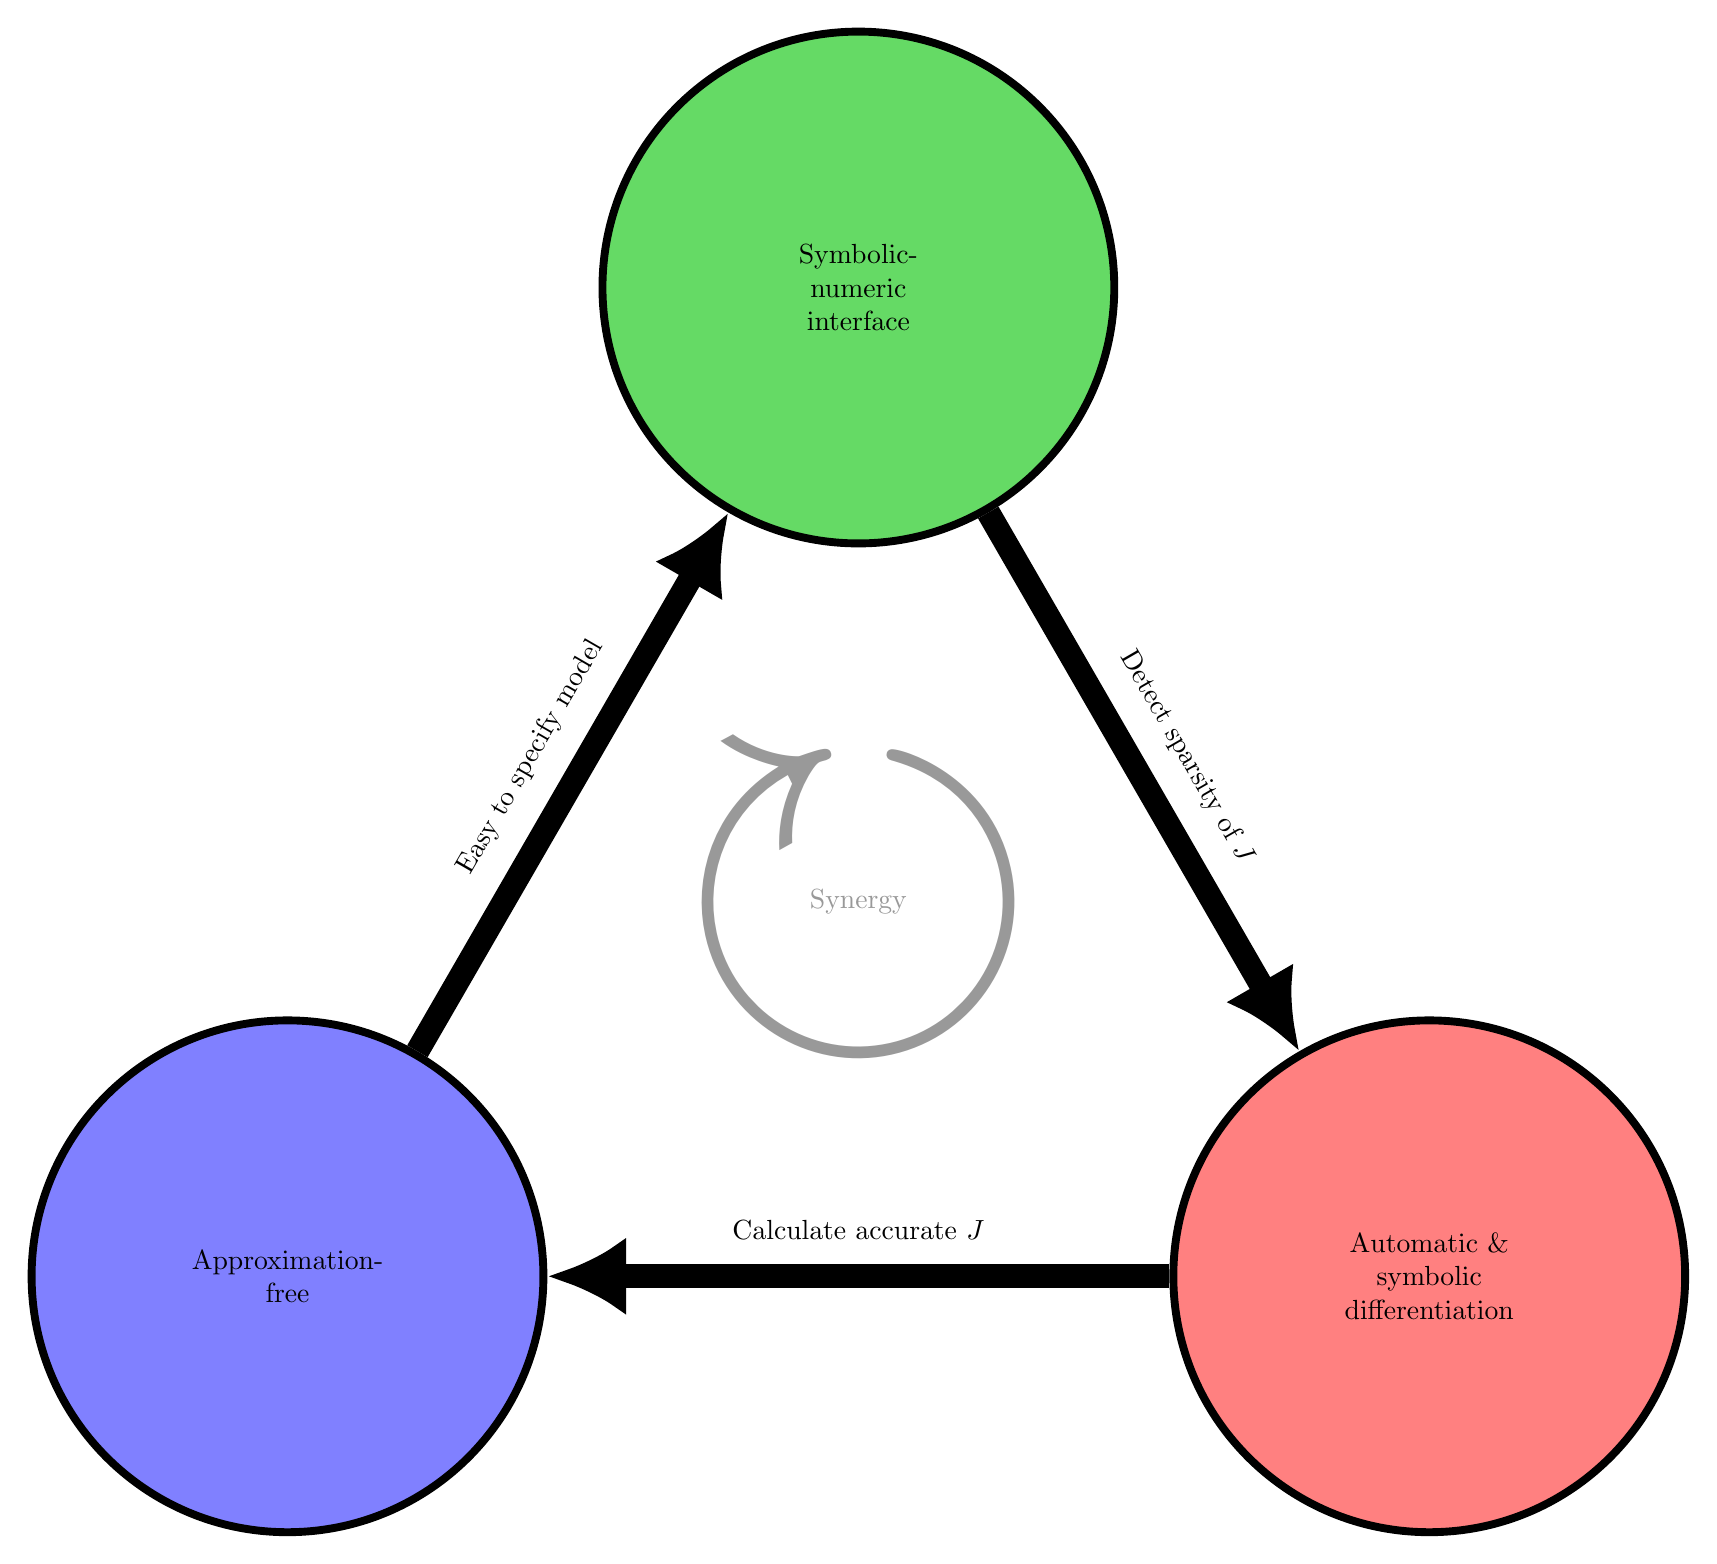
\begin{tikzpicture}[
        pillar/.style={circle, draw, minimum size=6.5cm, line width=1mm, align=center, font=\normalsize},
        joiner/.style={midway, sloped, black, font=\normalsize},
        arrow/.style={-{Latex[width=10mm,length=10mm]}, line width=3mm, black},
    ]
    \node[pillar, fill=LimeGreen!75] (sym) at (0:0cm) {Symbolic-\\numeric\\interface};
    \node[pillar, fill=blue!50] (app) at (240:14.5cm) {Approximation-\\free};
    \node[pillar, fill=red!50] (dif) at (300:14.5cm) {Automatic \&\\symbolic\\differentiation};
    \node[pillar, draw=none, black!40, font=\normalsize] (mid) at (270:7.8cm) {Synergy};
    \node[black!40, font=\fontsize{170pt}{170pt}, rotate=12.5] (rec) at (270:7.8cm) {$\circlearrowright$};
    %\draw[thick, black!50, -{Latex[length=6mm]}] (mid) ++(-45:3cm) arc[start angle=-45, end angle=315, radius=3cm];

    \draw[arrow] (sym.300) -- node[joiner, above=0.2cm] {Detect sparsity of $J$} (dif.120);
    \draw[arrow] (dif.180) -- node[joiner, above=0.2cm] {Calculate accurate $J$} (app.0);
    \draw[arrow] (app.60) -- node[joiner, above=0.2cm] {Easy to specify model} (sym.240);
    \end{tikzpicture}
    \end{center}
    \end{minipage}
    \bigskip

    \begin{itemize}
    \item \textbf{Symbolic-numeric:} Users enter symbolic equations $\rightarrow$ compiled to numerical code.
    \begin{itemize}
    \item Easier to modify eqs. than in CAMB \& CLASS. No need to dive into low-level code.
    %\item Users need not dive into the internals of the code.0
    \item Automates repetitive tasks, such as separation/splining of background/perturbations.
    %\item Full ΛCDM model (w/ RECFAST \& massive neutrinos) specified in 277 lines of code.
    \item Extra info to ODE solver, e.g. anal. Jacobian that is unknown in CAMB \& CLASS.
    \end{itemize}
    \item \textbf{Approximation-free:} Integrates full equations at all times with stiff ODE solvers.
    \begin{itemize}
    \item No TCA, UFA, RSA or NCDMFA, which significantly complicate CAMB \& CLASS.
    \item Much simpler: no need to rederive and recheck approximations for model extensions.
    \end{itemize}
    %\item \textbf{Fast:} Compiles symbolic equations into sparse \& analytical ODE Jacobians.
    %\begin{itemize}
 	%\item Maximizes speed \& stability for stiff solvers without extra user input.
    %\item Purely numerical codes like CAMB \& CLASS do not have this information!
    %\item SymBoltz (with no approx.) is $10\times$-$1\times$ faster than CLASS with approx. off/on.
    %\end{itemize}
    \item \textbf{Differentiable:} Compute $\partial(\mathrm{output})/\partial(\mathrm{input})$ with automatic differentiation.
    \begin{itemize}
	\item For example: $\partial P(k) / \partial \Omega_{m0}$, $\partial C_\ell^\text{TT} / \partial h$ or $\partial d_L(z) / \partial \Omega_{\Lambda 0}$.
    \item Uses numerically exact chain rules. No tuning of $\epsilon$ with finite differences.
    \item Useful for Fisher forecasting \& gradient-based MCMC (HMC) and optimization.
    \end{itemize}
    \end{itemize}
}

\block[bodyverticalshift=-1.5cm]{Simplicity: SymBoltz vs. CLASS}{
    \begin{center}
    \begin{minipage}[t]{0.49\linewidth}
    \begin{center}
    \vspace*{0mm}
    Massless neutrino equations in SymBoltz:
    \vspace{-0.6cm}
    \begin{codeinbox}[fontupper=\fontsize{8pt}{8pt}]
    \UseVerbatim{eqs_symboltz}
    \end{codeinbox}
    \end{center}
    \vspace{7.8cm}
    \begin{itemize}
    \item Similar difference for any part of eqs.
    \item Reason: symbolic-numeric \& no approx.
    \end{itemize}
    \bigskip\bigskip
    \begin{itemize}
    \item SymBoltz: full ΛCDM model in 277 lines.
    \item CLASS: spread over 27 000 lines \& 10 files.
    \end{itemize}
    \end{minipage}
    \hfill
    \begin{minipage}[t]{0.49\linewidth}
    \begin{center}
    \vspace*{0mm}
    Massless neutrino equations in CLASS:
    \vspace{-0.6cm}
    \begin{codeinbox}[fontupper=\fontsize{8pt}{8pt}]
    \UseVerbatim{eqs_class}
    \end{codeinbox}
    \end{center}
    \end{minipage}
    \end{center}
}

\block[bodyverticalshift=-2cm]{Accuracy: SymBoltz vs. CLASS}{
    \begin{center}
	
\includegraphics[width=\linewidth]{../../paper/figures/spectra.pdf}
    \end{center}
    \vspace{-0.8cm}
    \begin{itemize}
    \item Matter \& CMB power spectra agree around $\lesssim 0.1\,\%$ for default-ish precision parameters.
    \end{itemize}
}

\block[bodyverticalshift=-2cm]{Performance: SymBoltz vs. CLASS}{
	\begin{center}
    \begin{minipage}[t]{0.60\linewidth}
    \vspace*{0mm}
	\includegraphics[width=\linewidth]{../../paper/figures/work_precision.pdf}
    \end{minipage}
    \hfill
    \begin{minipage}[t]{0.39\linewidth}
    \vspace*{0mm}
    \bigskip
    $L_2$ error of $P(k)$ for perturbation ODE tolerances $10^{−9}$-$10^{−2}$ vs. $10^{−10}$ reference with different ODE solvers.
	Same $k$-modes \& $\ell_\text{max}$. Default massive neutrino sampling.
	\textbf{Lower left ($\boldsymbol{\swarrow}$) is better.}
    \newline
    \vspace{-0.5cm}
    \begin{itemize}
    \item SymBoltz is $10\times$/$1\times$ faster than CLASS with approx. off/on.
    \item Work in progress to optimize computation of CMB spectra.
    \end{itemize}
    \end{minipage}
    \end{center}
}

\iffalse
\block[bodyverticalshift=-1.75cm]{Implementation (\textcolor[HTML]{7CB342}{complete}/\textcolor[HTML]{FFCC32}{in progress}/\textcolor[HTML]{F44336}{planned})}{ % colors from dropper tool on emojis
    \small
    \begin{multicols}{3}
    \emoji{🟩} Baryons + photons (RECFAST) \\
    \emoji{🟩} Cold dark matter \\
    \emoji{🟩} Massless and massive neutrinos \\
    \emoji{🟩} Cosmological constant \\
    \emoji{🟨} Quintessence \\
    \emoji{🟩} $w_0 w_a$ dark energy \\
    \emoji{🟩} General Relativity \\
    \emoji{🟨} Brans-Dicke gravity \\
    \emoji{🟨} Curved geometry \\
    \emoji{🟩} Symbolic interface \\
    \emoji{🟩} Approximation-free (no TCA, RSA, UFA, \ldots) \\
    \emoji{🟩} Forward-mode automatic differentiation \\ 
    \emoji{🟩} Matter power spectrum \\
    \emoji{🟩} CMB power spectrum (TT, TE, EE) \\
    \emoji{🟩} Automatic stage separation ($\text{backgr.} \rightarrow \text{pert.}$) \\
    \emoji{🟩} Automatic splining of ODE unknowns \\
    \emoji{🟩} Automatic recomputation of ODE observeds \\
    \emoji{🟩} Automatic $(\tau,k)$-interpolation of any variable \\
    \emoji{🟨} Automatic series expansion of initial conditions \\
    \emoji{🟩} Automatic parameter assignment hooks \\
    \emoji{🟩} Shooting method for boundary conditions \\
    \emoji{🟩} Plot recipes (for convenient inspection) \\
    \emoji{🟨} Performance (isolate symbolics from numerics) \\
    \emoji{🟩} Extensive documentation pages \\
    \emoji{🟩} Continuous integration and testing \\
    \emoji{🟩} Comparison with \textsc{class} for ΛCDM \\
    \emoji{🟨} Non-linear: \textsc{halofit}/\textsc{hmcode} \\
    \emoji{🟥} Non-linear: generate $N$-body problems \\
    \emoji{🟥} Reverse-mode automatic differentiation \\
    \emoji{🟥} Automatic unit conversion utilities \\
    \emoji{🟥} Symbolic tensor manipulation \\
    \emoji{🟥} GPU parallellization \\
    \emoji{🟥} Better representation of interactions \\
    \emoji{🟨} Publication paper \\
    \emoji{⬛} \textbf{Ideas/contributions are very welcome!}
    \end{multicols}
}
\fi

\column{.50}

\block{Code example}{
    Install and launch \texttt{julia}. Load the package and build a standard ΛCDM model:
    \begin{codeinbox}
    \UseVerbatim{code1}
    \end{codeinbox}
    This is a \emph{symbolic} representation of all variables and equations in the model.
    It can be inspected and modified, for example to see the equations in the gravity component \enquote{\texttt{G}}:
    \begin{codeinbox}
    \UseVerbatim{code2}
    \end{codeinbox}
    \vspace{-1cm}
    \begin{align}
    \frac{\mathrm{d} ~ a\left( \tau \right)}{\mathrm{d}\tau} &= \left( a\left( \tau \right) \right)^{2} ~ \sqrt{\frac{8}{3} ~ \pi ~ \rho\left( \tau \right)} \\
    \frac{\mathrm{d}}{\mathrm{d}\tau} ~ \Phi\left( \tau, k \right) &= \frac{ - k^{2} ~ \Phi\left( \tau, k \right)}{3 ~ \mathscr{H}\left( \tau \right)} + \frac{ - \frac{4}{3} ~ \left( a\left( \tau \right) \right)^{2} ~ \pi ~ \mathtt{\delta\rho}\left( \tau, k \right)}{\mathscr{H}\left( \tau \right)} - \mathscr{H}\left( \tau \right) ~ \Psi\left( \tau, k \right) \\
    k^{2} ~ \left( \Phi\left( \tau, k \right) - \Psi\left( \tau, k \right) \right) &= 12 ~ \left( a\left( \tau \right) \right)^{2} ~ \pi ~ \Pi\left( \tau, k \right)
    \end{align}
    Now set cosmological parameters and compile the symbolic model to a \emph{numerical} problem:
    \begin{codeinbox}
    \UseVerbatim{code3}
    \end{codeinbox}
    This performs several automatic steps: splitting equations into background \& perturbations, splining background variables needed by the perturbations, generating ODE functions \& Jacobians, etc.
    We can solve the background \& perturbations for any $k$-modes:
    \begin{codeinbox}
    \UseVerbatim{code4}
    \end{codeinbox}
    The solution object can easily get or plot \emph{any} symbolic expression as a function of $(\tau, k)$:
    \begin{codeinbox}
    \UseVerbatim{code5}
    \end{codeinbox}
    \begin{center}
    \includegraphics[width=0.33\linewidth]{../../notebooks/poster2/plot1.pdf}\hfill%
    \includegraphics[width=0.33\linewidth]{../../notebooks/poster2/plot2.pdf}\hfill%
    \includegraphics[width=0.33\linewidth]{../../notebooks/poster2/plot3.pdf}\\
    \end{center}
    Compute matter and CMB power spectra (keyword arguments control precision settings):
    \begin{codeinbox}
    \UseVerbatim{code6}
    \end{codeinbox}
    Implement a new $w_0 w_a$ dark energy component (with much less work than in other codes):
    \begin{codeinbox}
    \UseVerbatim{code7}
    \end{codeinbox}
    %Modification to \emph{any} sector of the equations is equally simple.
}

% https://tex.stackexchange.com/a/183867
\block[bodyverticalshift=-0.3cm]{\huge Installation and documentation}{
\noindent
\hspace{1cm}
\begin{minipage}{0.30\linewidth}
    \qrcode[height=10cm]{https://github.com/hersle/SymBoltz.jl}
\end{minipage}%
\hfill%
\begin{adjustbox}{valign=c}%
\begin{minipage}{0.70\linewidth}
    \LARGE Easy to install with one command, see:
    \begin{quote}
        \LARGE \textcolor{blue}{\url{github.com/hersle/SymBoltz.jl}}
    \end{quote}
    \textbf{Feedback is greatly appreciated.}\\
    \textbf{Open an issue to get in touch!}
\end{minipage}
\end{adjustbox}
\vspace{1cm}
}

\end{columns}

\end{document}
